\documentclass[a4paper,12pt]{article}

\usepackage[utf8]{inputenc}
\usepackage[T5]{fontenc}
\usepackage[vietnamese]{babel}
\usepackage{amsmath,amssymb}
\usepackage{graphicx}
\usepackage{booktabs}
\usepackage{longtable}
\usepackage{array}
\usepackage{tabularx}
\usepackage{multirow}
\usepackage{float}
\usepackage{setspace}
\usepackage{geometry}
\usepackage{caption}
\usepackage{enumitem}
\usepackage{fancyhdr}
\usepackage{lastpage}
\usepackage{xcolor}
\usepackage{url}
\usepackage{hyperref}
\usepackage{tocloft}
\usepackage{tikz}
\usetikzlibrary{shapes.geometric, arrows, positioning}

\geometry{left=2.7cm,right=2.7cm,top=2.5cm,bottom=2.5cm}
\setstretch{1.25}
\graphicspath{{figures/}}

\AtBeginDocument{\renewcommand*\contentsname{Mục lục}}
\AtBeginDocument{\renewcommand*\listfigurename{Danh mục hình vẽ}}
\AtBeginDocument{\renewcommand*\listtablename{Danh mục bảng biểu}}
\AtBeginDocument{\renewcommand*\refname{Tài liệu tham khảo}}

\hypersetup{
    colorlinks=true,
    linkcolor=black,
    citecolor=black,
    urlcolor=blue,
    pdfborder={0 0 0}
}

\setlength{\headheight}{35pt}
\pagestyle{fancy}
\fancyhead{}
\fancyhead[L]{
\begin{tabular}{rl}
\begin{picture}(25,15)(0,0)
\put(0,-8){
\includegraphics[width=8mm,height=8mm]{hcmut.png}}
\end{picture}
&
\begin{tabular}{l}
\small \textbf{\ttfamily Trường Đại học Bách khoa -- ĐHQG-HCM}\\
\small \textbf{\ttfamily Khoa Khoa học và Kỹ thuật Máy tính}
\end{tabular}
\end{tabular}
}
\fancyhead[R]{\small \ttfamily Học máy -- HK2 2025-2026}
\fancyfoot{}
\fancyfoot[L]{\scriptsize \ttfamily Báo cáo bài tập lớn môn Học máy}
\fancyfoot[R]{\scriptsize \ttfamily Trang \thepage/\pageref{LastPage}}
\renewcommand{\headrulewidth}{0.3pt}
\renewcommand{\footrulewidth}{0.3pt}

\setcounter{secnumdepth}{3}
\setcounter{tocdepth}{2}

\begin{document}

\begin{titlepage}
\begin{center}
\textbf{ĐẠI HỌC QUỐC GIA THÀNH PHỐ HỒ CHÍ MINH} \\
\textbf{TRƯỜNG ĐẠI HỌC BÁCH KHOA} \\
\textbf{KHOA KHOA HỌC VÀ KỸ THUẬT MÁY TÍNH}
\end{center}

\vspace{1cm}

\begin{figure}[H]
\centering

\includegraphics[width=3.0cm]{hcmut.png}
\end{figure}

\vspace{0.8cm}

\begin{center}
\begin{tabular}{c}
\multicolumn{1}{c}{\textbf{\LARGE HỌC MÁY (CO3061)}} \\
~~\\
\hline
\\
\multicolumn{1}{c}{\textbf{\Large BÁO CÁO BÀI TẬP LỚN}} \\
\\
\textbf{\large \MakeUppercase{Xây dựng pipeline phân loại văn bản}} \\
\textbf{\large \MakeUppercase{CFPB Consumer Complaints}} \\
\\
\hline
\end{tabular}
\end{center}

\vspace{0.8cm}

\begin{table}[H]
\centering
\begin{tabular}{r l}
\textbf{Giảng viên hướng dẫn:} & [Điền tên GVHD] \\
\textbf{Nhóm thực hiện:} & [Điền thành viên 1 -- MSSV] \\
& [Điền thành viên 2 -- MSSV] \\
& [Điền thành viên 3 -- MSSV] \\
\end{tabular}
\end{table}

\vfill
\begin{center}
TP. Hồ Chí Minh -- 2026
\end{center}
\end{titlepage}

\thispagestyle{empty}
\newpage
\tableofcontents
\thispagestyle{empty}
\newpage
\listoffigures
\addcontentsline{toc}{section}{Danh mục hình vẽ}
\thispagestyle{empty}
\newpage
\listoftables
\addcontentsline{toc}{section}{Danh mục bảng biểu}
\thispagestyle{empty}
\newpage
\pagenumbering{arabic}
\setcounter{page}{1}

\section*{Lời nói đầu}
\addcontentsline{toc}{section}{Lời nói đầu}

Bài tập lớn môn Học máy yêu cầu triển khai trọn vẹn một pipeline học máy truyền thống cho dữ liệu văn bản, bao gồm các bước từ EDA, tiền xử lý, trích xuất đặc trưng, huấn luyện mô hình đến đánh giá kết quả. Trong báo cáo này, nhóm thực hiện bài toán phân loại khiếu nại người tiêu dùng tài chính từ bộ dữ liệu CFPB theo 7 nhóm sản phẩm chính.

Pipeline được tổ chức theo hướng module hóa nhằm đảm bảo khả năng tái sử dụng và mở rộng: module tiền xử lý văn bản, module trích xuất đặc trưng, module huấn luyện/đánh giá, cùng notebook tổng hợp thực nghiệm. Bên cạnh các đặc trưng truyền thống (BoW, TF-IDF), nhóm bổ sung hai hướng embedding hiện đại (Word2Vec và BERT sentence embeddings) để so sánh định lượng, qua đó đáp ứng cả yêu cầu bắt buộc và phần khuyến khích của đề bài.

Bố cục của báo cáo được tổ chức thành 4 phần chính:
\begin{enumerate}[nosep]
    \item \textbf{Cơ sở lý thuyết và phát biểu bài toán:} Trình bày mục tiêu, dữ liệu và nền tảng các phương pháp sử dụng.
    \item \textbf{Thiết kế và hiện thực hệ thống:} Kiến trúc pipeline, quy trình tiền xử lý và các kỹ thuật trích xuất đặc trưng.
    \item \textbf{Kết quả thực nghiệm và phân tích:} Phân tích số liệu định lượng, so sánh các mô hình và đánh giá hiệu năng chi tiết.
    \item \textbf{Kết luận và hướng phát triển:} Tổng kết các kết quả chính và đề xuất hướng mở rộng.
\end{enumerate}

\newpage
\section{Cơ sở lý thuyết và phát biểu bài toán}

\subsection{Phát biểu bài toán}
Mục tiêu của dự án là xây dựng pipeline học máy để \textbf{phân loại nội dung khiếu nại tài chính} từ bộ dữ liệu CFPB (Consumer Financial Protection Bureau) vào các nhóm sản phẩm. Bài toán được mô hình hóa dưới dạng phân loại đa lớp:
\begin{equation}
\hat{y} = f(x), \quad y \in \{1,\ldots,K\}, \ K=7
\end{equation}
trong đó $x$ là văn bản khiếu nại, $y$ là nhãn sản phẩm tài chính tương ứng.

Theo yêu cầu học phần, hệ thống cần bao phủ đầy đủ các bước của pipeline truyền thống: EDA, tiền xử lý, trích xuất đặc trưng, huấn luyện và đánh giá. Đồng thời, nhóm mở rộng thêm embedding hiện đại (Word2Vec, BERT) để so sánh với đặc trưng truyền thống.

\subsection{Bộ dữ liệu và chiến lược lấy mẫu}
\subsubsection{Nguồn dữ liệu}
Dữ liệu được tải từ cổng công khai CFPB\footnote{\url{https://files.consumerfinance.gov/ccdb/complaints.csv.zip}}. File gốc có kích thước lớn, vì vậy notebook sử dụng cơ chế đọc theo từng khối (chunked reading) để tránh quá tải bộ nhớ.

\subsubsection{Tiêu chí lọc và chuẩn hóa nhãn}
Từ dữ liệu thô, nhóm áp dụng các bước:
\begin{itemize}[nosep]
    \item Chỉ giữ mẫu có \texttt{Consumer complaint narrative} không rỗng và đủ dài.
    \item Chuẩn hóa các nhãn \texttt{Product} thay đổi theo thời gian về tập nhãn thống nhất.
    \item Loại các lớp có kích thước quá nhỏ, sau đó giữ top-7 lớp nhiều mẫu nhất.
    \item Lấy mẫu cân bằng theo lớp, kết hợp lọc hậu tiền xử lý (văn bản quá ngắn).
\end{itemize}

Kết quả sau xử lý sạch hiện có 13{,}983 mẫu, phân bố gần cân bằng như Bảng~\ref{tab:class_dist}.

\begin{table}[H]
\centering
\caption{Phân bố nhãn trong dữ liệu sạch hiện tại}
\label{tab:class_dist}
\begin{tabular}{lrr}
\toprule
\textbf{Nhãn} & \textbf{Số mẫu} & \textbf{Tỷ lệ (\%)} \\
\midrule
Bank account & 1{,}998 & 14.29 \\
Credit card & 1{,}999 & 14.30 \\
Credit reporting & 1{,}993 & 14.25 \\
Debt collection & 1{,}995 & 14.27 \\
Money transfer & 1{,}998 & 14.29 \\
Mortgage & 2{,}000 & 14.30 \\
Student loan & 2{,}000 & 14.30 \\
\midrule
\textbf{Tổng} & \textbf{13{,}983} & \textbf{100.00} \\
\bottomrule
\end{tabular}
\end{table}

\subsection{Pipeline tiền xử lý văn bản}
Pipeline tiền xử lý được triển khai trong module \texttt{text\_preprocessor.py}, gồm các bước chính:
\begin{enumerate}[nosep]
    \item Chuẩn hóa Unicode và chuyển chữ thường.
    \item Loại URL, email.
    \item Chuẩn hóa số tiền thành token \texttt{moneytok}.
    \item Loại token bị ẩn danh dạng \texttt{XX...} và chữ số.
    \item Loại dấu câu, chuẩn hóa khoảng trắng.
    \item Tokenization, loại stopwords, lemmatization.
\end{enumerate}

Sau tiền xử lý, độ dài văn bản (số từ) có trung bình 96.90, trung vị 65, tứ phân vị trên 118 và giá trị lớn nhất 2{,}649 từ.

\subsection{Các phương pháp trích xuất đặc trưng}
\subsubsection{Đặc trưng truyền thống}
\textbf{Bag-of-Words (BoW)} biểu diễn văn bản bằng tần suất từ trong từ điển. \textbf{TF-IDF} được dùng ở hai cấu hình: unigram và bigram. Trọng số TF-IDF của từ $t$ trong văn bản $d$:
\begin{equation}
\mathrm{tfidf}(t,d) = \mathrm{tf}(t,d) \cdot \log\frac{N}{\mathrm{df}(t)}
\end{equation}
trong đó $N$ là số văn bản huấn luyện, $\mathrm{df}(t)$ là số văn bản chứa từ $t$.

\subsubsection{Đặc trưng hiện đại}
\textbf{Word2Vec}: huấn luyện embedding trên corpus, sau đó lấy trung bình vector từ để tạo vector văn bản:
\begin{equation}
\mathbf{v}_{doc} = \frac{1}{|S|}\sum_{w \in S}\mathbf{v}_w
\end{equation}
trong đó $S$ là tập từ hợp lệ trong văn bản.

\textbf{BERT sentence embeddings}: sử dụng \texttt{all-MiniLM-L6-v2} (384 chiều), encode trực tiếp văn bản (đã cắt ngắn để giảm thời gian suy diễn).

\subsection{Mô hình phân loại và chỉ số đánh giá}
Các mô hình trong thực nghiệm được lựa chọn dựa trên đặc thù của dữ liệu văn bản:
\begin{itemize}[nosep]
    \item \textbf{Naive Bayes (Multinomial \& Complement):} Phù hợp với đặc trưng tần suất từ (BoW, TF-IDF). Complement NB đặc biệt hiệu quả với dữ liệu có sự mất cân bằng nhẹ.
    \item \textbf{Logistic Regression:} Mô hình baseline mạnh mẽ cho bài toán phân loại văn bản, dễ giải thích trọng số của từng từ.
    \item \textbf{LinearSVC (Support Vector Classification):} Hiệu quả cao trong không gian đặc trưng có số chiều lớn (như TF-IDF bigram).
    \item \textbf{Random Forest:} Mô hình ensemble giúp đánh giá hiệu năng của phương pháp phi tuyến tính trên dữ liệu văn bản.
\end{itemize}

Với bài toán đa lớp, các chỉ số chính:
\begin{equation}
\mathrm{Accuracy} = \frac{\text{số dự đoán đúng}}{\text{tổng số mẫu}}
\end{equation}
\begin{equation}
\mathrm{Precision} = \frac{TP}{TP+FP},\quad
\mathrm{Recall} = \frac{TP}{TP+FN},\quad
F1 = \frac{2PR}{P+R}
\end{equation}
Báo cáo sử dụng \textbf{F1-weighted} làm tiêu chí xếp hạng chính vì phản ánh đồng thời độ chính xác và mức cân bằng theo lớp.

\subsection{Định hướng thiết kế thực nghiệm}
Thiết kế thực nghiệm theo nguyên tắc:
\begin{itemize}[nosep]
    \item So sánh công bằng nhiều loại đặc trưng trên cùng tập train/test.
    \item Chỉ dùng mô hình phù hợp miền dữ liệu (ví dụ NB cho đặc trưng không âm).
    \item Tuning tham số $C$ cho Logistic Regression và LinearSVC trên đặc trưng mạnh nhất.
    \item Lưu toàn bộ đặc trưng và kết quả để tái lập thí nghiệm.
\end{itemize}

\newpage
\section{Thiết kế và hiện thực hệ thống}

\subsection{Kiến trúc triển khai}
Hệ thống được tổ chức theo kiến trúc module, tách biệt xử lý dữ liệu, trích xuất đặc trưng và huấn luyện mô hình. Cấu trúc chính gồm:
\begin{itemize}[nosep]
    \item \texttt{modules/text\_preprocessor.py}: tiền xử lý văn bản.
    \item \texttt{modules/feature\_extractor.py}: trích xuất BoW, TF-IDF, Word2Vec, BERT.
    \item \texttt{modules/trainer.py}: huấn luyện, đánh giá, tổng hợp chỉ số.
    \item \texttt{notebooks/main\_pipeline.ipynb}: orchestrate toàn bộ thí nghiệm.
    \item \texttt{reports/experiment\_results.csv}: lưu bảng kết quả cuối.
\end{itemize}

\begin{figure}[H]
\centering
\begin{tikzpicture}[node distance=1.5cm and 2cm, auto,
    block/.style={rectangle, draw, fill=blue!10, text width=2.8cm, text centered, rounded corners, minimum height=1.2cm},
    data/.style={cylinder, draw, shape border rotate=90, fill=gray!10, text width=1.8cm, text centered, minimum height=1.2cm},
    arrow/.style={thick,->,>=stealth}]

    % Nodes
    \node [data] (raw) {Raw Data};
    \node [block, right=of raw] (prep) {Text Preprocessor};
    \node [block, right=of prep] (feat) {Feature Extractor};
    \node [block, below=of feat, yshift=-0.5cm] (train) {Model Trainer};
    \node [data, below=of prep, yshift=-0.5cm] (results) {Reports};

    % Arrows
    \draw [arrow] (raw) -- (prep);
    \draw [arrow] (prep) -- (feat);
    \draw [arrow] (feat) -- (train);
    \draw [arrow] (train) -- (results);
    
\end{tikzpicture}
\caption{Kiến trúc tổng quan của pipeline phân loại văn bản}
\label{fig:architecture}
\end{figure}

Thiết kế này giúp thay thế từng thành phần độc lập mà không làm ảnh hưởng các phần còn lại, phù hợp yêu cầu "pipeline có thể cấu hình" của đề bài.

\subsection{Tiền xử lý văn bản}
Pipeline tiền xử lý được gọi theo chuỗi:
\begin{equation}
\text{clean} \rightarrow \text{tokenize} \rightarrow \text{remove stopwords} \rightarrow \text{lemmatize}
\end{equation}

Trong bước \texttt{clean}, hệ thống xử lý các đặc thù của CFPB narratives:
\begin{itemize}[nosep]
    \item Loại URL, email, số và dấu câu.
    \item Chuẩn hóa token tiền tệ thành \texttt{moneytok}.
    \item Loại token ẩn danh dạng \texttt{XX...} thường gặp trong dữ liệu khiếu nại.
\end{itemize}

Xử lý hàng loạt được song song hóa bằng \texttt{joblib.Parallel} để giảm thời gian tiền xử lý trên tập dữ liệu lớn.

\subsection{Trích xuất đặc trưng}
\subsubsection{Đặc trưng truyền thống}
Hai họ đặc trưng sparse được triển khai bằng \texttt{scikit-learn} \cite{scikit-learn}:
\begin{itemize}[nosep]
    \item BoW: \texttt{CountVectorizer(max\_features=30000, min\_df=2)}.
    \item TF-IDF unigram: \texttt{TfidfVectorizer(ngram\_range=(1,1), max\_features=30000, min\_df=2)}.
    \item TF-IDF bigram: \texttt{TfidfVectorizer(ngram\_range=(1,2), max\_features=50000, min\_df=2)}.
\end{itemize}

\subsubsection{Đặc trưng hiện đại}
\begin{itemize}[nosep]
    \item Word2Vec \cite{mikolov2013efficient}: huấn luyện trên tập train với \texttt{vector\_size=200, epochs=10}, sau đó lấy trung bình vector từ để tạo vector văn bản.
    \item BERT sentence embedding: \texttt{all-MiniLM-L6-v2} từ \texttt{sentence-transformers} \cite{reimers2019sentencebert}. Văn bản đầu vào được cắt còn 150 từ, model encode ở \texttt{max\_length=128} để cân bằng chất lượng và tốc độ.
\end{itemize}

Toàn bộ đặc trưng được lưu lại dưới dạng \texttt{.npz} (sparse) hoặc \texttt{.npy} (dense) để tái sử dụng giữa các lần chạy.

\subsection{Thiết lập huấn luyện và đánh giá}
Dữ liệu được chia train/test theo tỉ lệ 80/20 có stratify theo nhãn. Trên artifact hiện hành:
\begin{equation}
|\mathcal{D}_{train}| = 11{,}184, \quad |\mathcal{D}_{test}| = 2{,}797
\end{equation}

Các mô hình được huấn luyện:
\begin{itemize}[nosep]
    \item Complement Naive Bayes, Multinomial Naive Bayes.
    \item Logistic Regression (solver \texttt{saga}, \texttt{max\_iter=1000}).
    \item LinearSVC (\texttt{max\_iter=2000}).
    \item Random Forest (\texttt{n\_estimators=50}, \texttt{max\_features=sqrt}).
\end{itemize}

Tổng số cấu hình được ghi nhận trong báo cáo kết quả là 20 dòng: 18 cấu hình gốc và 2 cấu hình sau tuning.

\subsection{Ma trận thí nghiệm}
Bảng~\ref{tab:exp_matrix} mô tả phạm vi mô hình theo từng nhóm đặc trưng.

\begin{table}[H]
\centering
\caption{Ma trận thực nghiệm}
\label{tab:exp_matrix}
\begin{tabular}{lccccc}
\toprule
\textbf{Feature} & \textbf{C-NB} & \textbf{M-NB} & \textbf{LR} & \textbf{SVM} & \textbf{RF} \\
\midrule
BoW & \checkmark & \checkmark & \checkmark & \checkmark & \checkmark \\
TF-IDF Unigram & \checkmark & \checkmark & \checkmark & \checkmark & \checkmark \\
TF-IDF Bigram & \checkmark &  & \checkmark & \checkmark & \checkmark \\
Word2Vec &  &  & \checkmark & \checkmark &  \\
BERT (MiniLM) &  &  & \checkmark & \checkmark &  \\
\bottomrule
\end{tabular}
\end{table}

Lý do loại trừ một số tổ hợp:
\begin{itemize}[nosep]
    \item Naive Bayes chỉ phù hợp với đặc trưng không âm (BoW/TF-IDF).
    \item Random Forest không được ưu tiên trên embedding dense vì chi phí tính toán cao và hiệu quả không nổi bật trong benchmark hiện tại.
\end{itemize}

\subsection{Hyperparameter tuning}
Tuning được thực hiện trên feature mạnh nhất (TF-IDF bigram) với lưới:
\begin{equation}
C \in \{0.01,\ 0.1,\ 0.5,\ 1.0,\ 5.0,\ 10.0\}
\end{equation}
Dùng 3-fold CV với tiêu chí \texttt{f1\_weighted} để chọn tham số tốt nhất. Kết quả chọn:
\begin{equation}
C_{\text{best,LR}} = 5.0, \quad C_{\text{best,SVM}} = 0.5
\end{equation}

\subsection{Kiểm thử mã nguồn}
Bộ kiểm thử đơn vị đã được viết cho ba module chính trong thư mục \texttt{tests/}. Các ca kiểm thử bao phủ:
\begin{itemize}[nosep]
    \item Tính đúng đắn của bước làm sạch văn bản và pipeline tiền xử lý.
    \item Tính nhất quán shape dữ liệu khi build/save/load đặc trưng.
    \item Tính đầy đủ chỉ số trả về của hàm huấn luyện và sắp xếp bảng tổng hợp.
\end{itemize}



\newpage
\section{Kết quả thực nghiệm và phân tích}

\subsection{Tổng quan dữ liệu sau tiền xử lý}
Dữ liệu sạch hiện tại trong \texttt{data/df\_clean.parquet} gồm 13{,}983 mẫu, 7 lớp cân bằng gần đều. Độ dài văn bản sau tiền xử lý có đặc trưng:
\begin{equation}
\mu=96.90,\ \mathrm{median}=65,\ Q_1=36,\ Q_3=118,\ \max=2649\ \text{(từ)}
\end{equation}

Hình~\ref{fig:label_dist} và Hình~\ref{fig:text_len} minh họa phân phối nhãn và độ dài văn bản.

\begin{figure}[H]
\centering
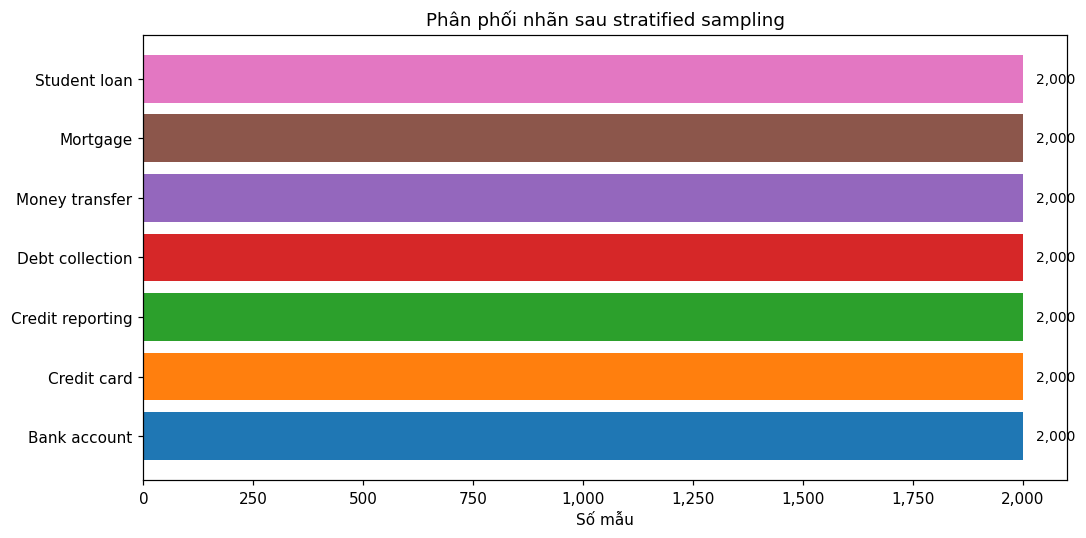
\includegraphics[width=0.85\textwidth]{01_label_distribution.png}
\caption{Phân phối nhãn sau lấy mẫu và làm sạch}
\label{fig:label_dist}
\end{figure}

\begin{figure}[H]
\centering
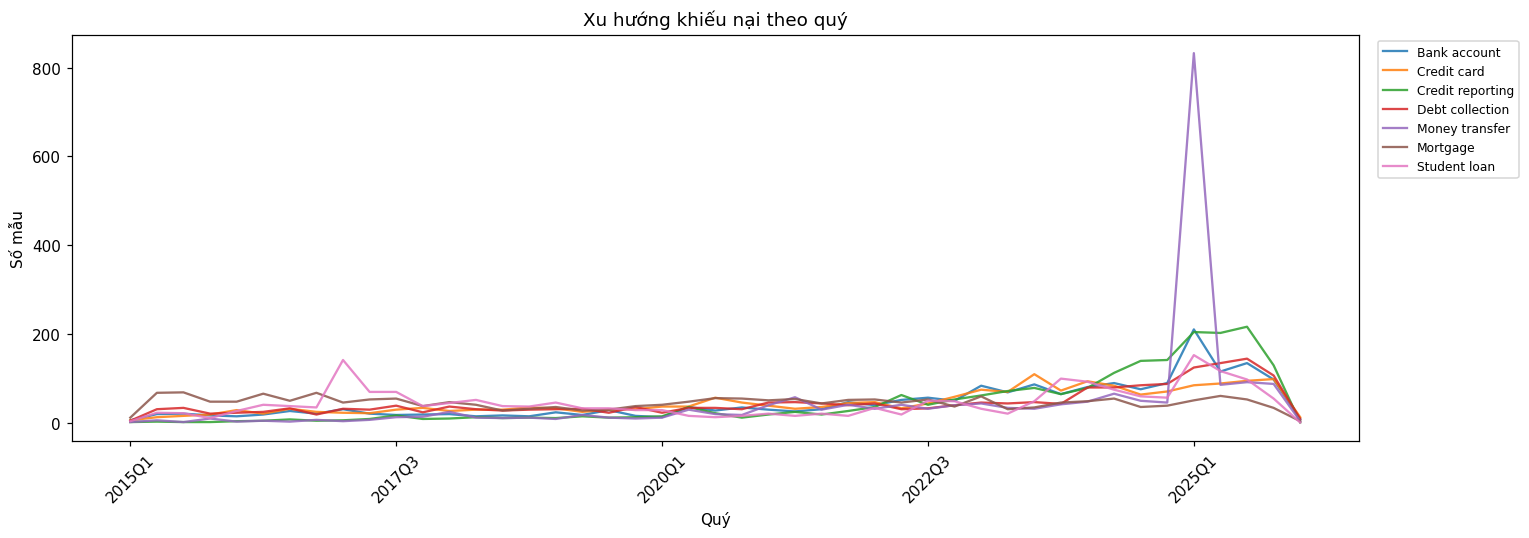
\includegraphics[width=0.85\textwidth]{05_time_trend.png}
\caption{Xu hướng số lượng khiếu nại theo thời gian (tháng/năm)}
\label{fig:time_trend}
\end{figure}

\begin{figure}[H]
\centering
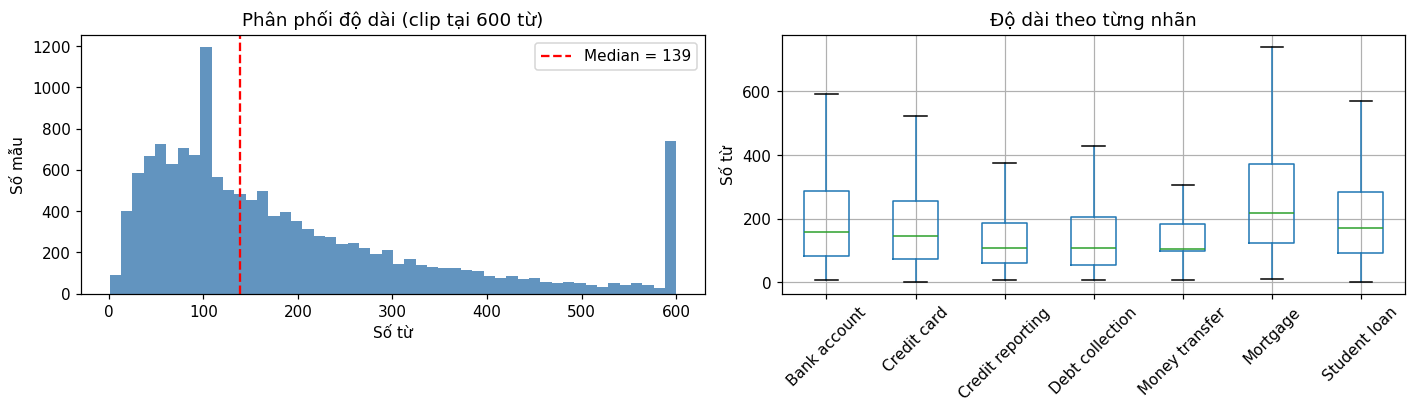
\includegraphics[width=0.95\textwidth]{02_text_length.png}
\caption{Phân phối độ dài văn bản và boxplot theo nhãn}
\label{fig:text_len}
\end{figure}

\begin{figure}[H]
\centering
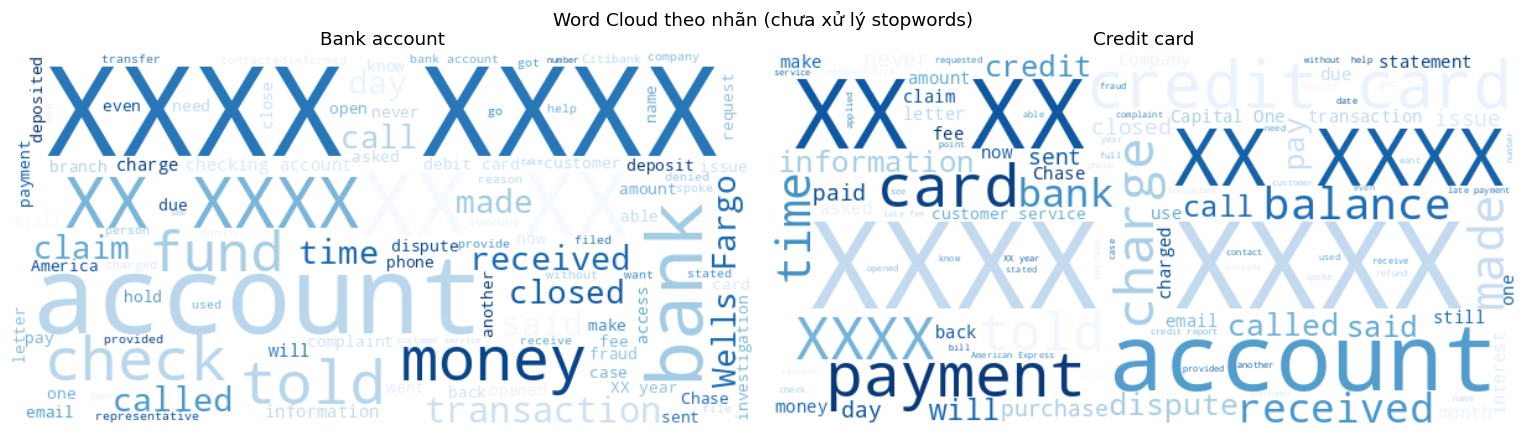
\includegraphics[width=0.95\textwidth]{04_wordcloud.png}
\caption{Word Cloud của các từ phổ biến nhất sau khi tiền xử lý}
\label{fig:wordcloud}
\end{figure}

\begin{figure}[H]
\centering
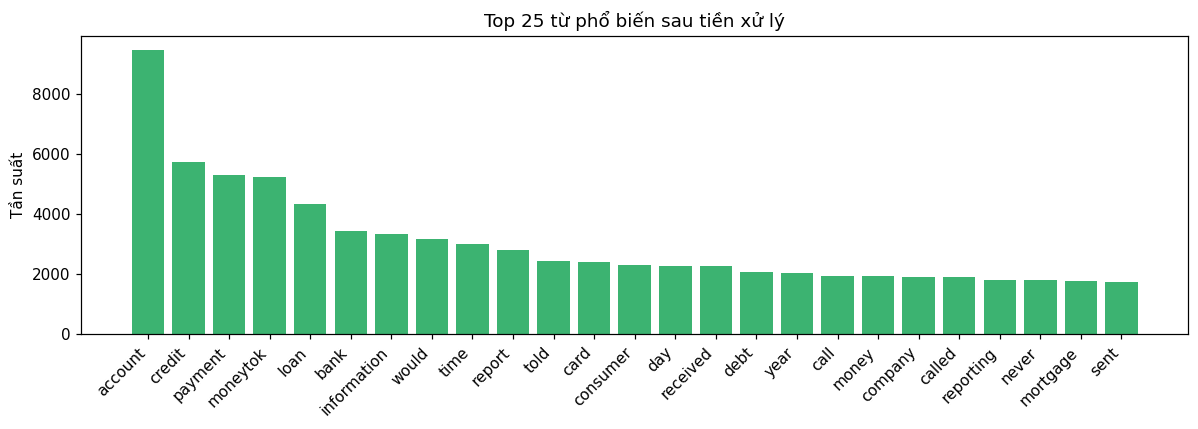
\includegraphics[width=0.95\textwidth]{06_top25_words_after_preprocess.png}
\caption{Top 25 từ xuất hiện nhiều nhất trong bộ dữ liệu}
\label{fig:top_words}
\end{figure}

\begin{figure}[H]
\centering
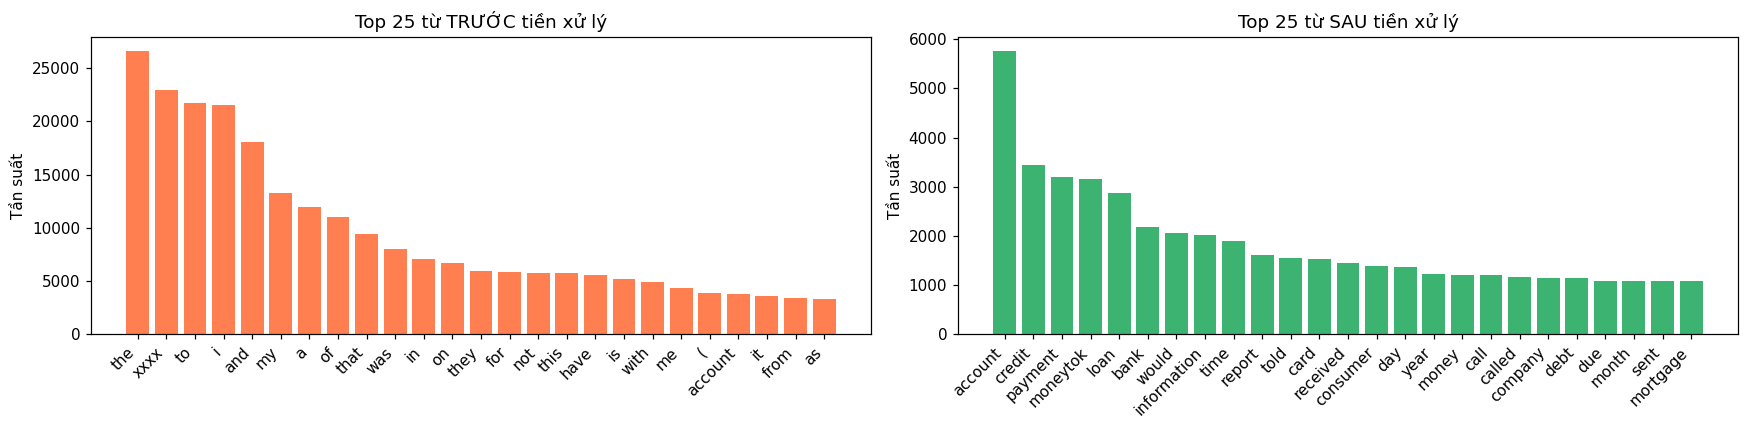
\includegraphics[width=0.95\textwidth]{03_word_freq_before_after.png}
\caption{So sánh tần suất từ trước và sau khi tiền xử lý (loại bỏ stopwords và làm sạch)}
\label{fig:word_freq_comp}
\end{figure}



\subsection{Kích thước các không gian đặc trưng}
\begin{table}[H]
\centering
\caption{Kích thước đặc trưng train/test từ artifact huấn luyện}
\label{tab:feature_shape}
\begin{tabular}{lcc}
\toprule
\textbf{Đặc trưng} & \textbf{Train shape} & \textbf{Test shape} \\
\midrule
BoW & (11184, 10254) & (2797, 10254) \\
TF-IDF Unigram & (11184, 10254) & (2797, 10254) \\
TF-IDF Bigram & (11184, 50000) & (2797, 50000) \\
Word2Vec & (11184, 200) & (2797, 200) \\
BERT (MiniLM) & (11184, 384) & (2797, 384) \\
\bottomrule
\end{tabular}
\end{table}

\subsection{Kết quả tổng hợp các mô hình}
Bảng~\ref{tab:top10} trình bày 10 cấu hình tốt nhất theo F1-weighted từ file \texttt{reports/experiment\_results.csv}.

\begin{table}[H]
\centering
\caption{Top-10 cấu hình theo F1-weighted}
\label{tab:top10}
\begin{tabular}{p{3.4cm}p{2.6cm}ccc}
\toprule
\textbf{Feature} & \textbf{Model} & \textbf{Acc.} & \textbf{F1-w} & \textbf{Time (s)} \\
\midrule
TF-IDF Bigram (C=0.5) & SVM & 0.8631 & 0.8631 & 0.58 \\
TF-IDF Bigram & SVM & 0.8598 & 0.8599 & 0.75 \\
TF-IDF Bigram (C=5.0) & Logistic Regression & 0.8595 & 0.8597 & 2.23 \\
TF-IDF Unigram & Logistic Regression & 0.8588 & 0.8590 & 0.74 \\
TF-IDF Bigram & Logistic Regression & 0.8570 & 0.8573 & 1.22 \\
TF-IDF Unigram & SVM & 0.8441 & 0.8440 & 0.78 \\
TF-IDF Bigram & Complement NB & 0.8380 & 0.8374 & 0.02 \\
BoW & Logistic Regression & 0.8298 & 0.8305 & 39.55 \\
TF-IDF Unigram & Random Forest & 0.8291 & 0.8294 & 4.16 \\
TF-IDF Bigram & Random Forest & 0.8270 & 0.8270 & 7.70 \\
\bottomrule
\end{tabular}
\end{table}

Cấu hình tốt nhất toàn cục là \textbf{TF-IDF Bigram + LinearSVC (C=0.5)} với:
\begin{equation}
\mathrm{Accuracy}=0.8631,\ \mathrm{F1}_{macro}=0.8631,\ \mathrm{F1}_{weighted}=0.8631
\end{equation}

Hình~\ref{fig:f1_grouped} cho thấy xu hướng chung: họ TF-IDF, đặc biệt bigram, chiếm ưu thế rõ rệt.

\begin{figure}[H]
\centering
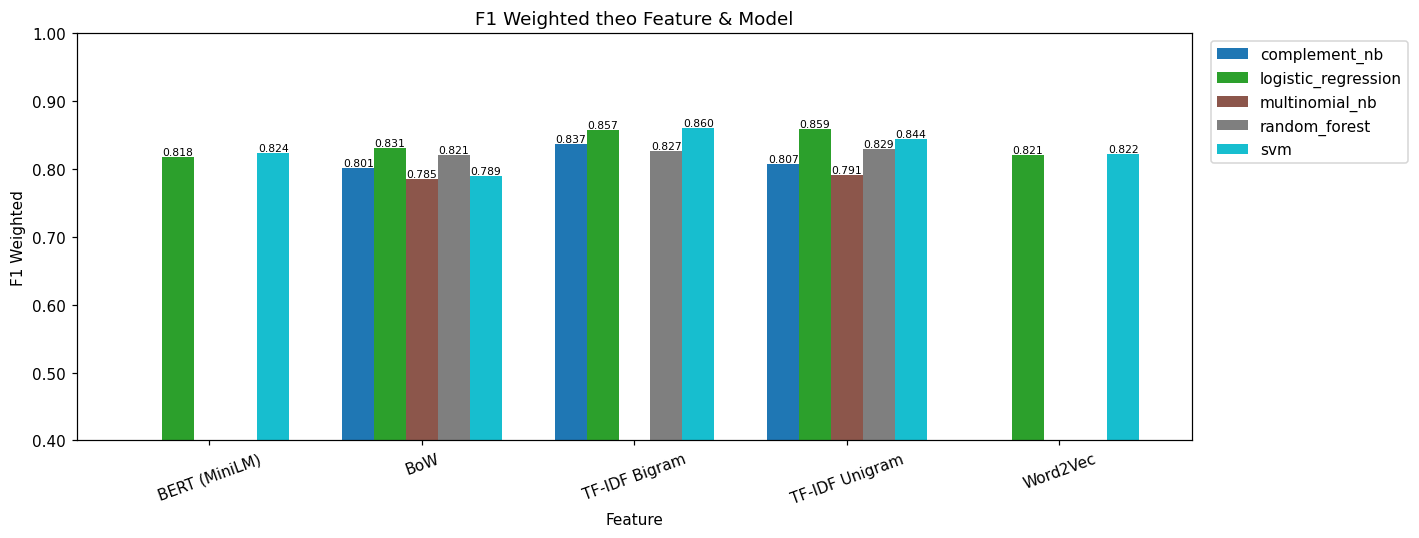
\includegraphics[width=\textwidth]{08_f1_grouped_bar.png}
\caption{So sánh F1-weighted theo đặc trưng và mô hình}
\label{fig:f1_grouped}
\end{figure}

\subsection{So sánh truyền thống và embedding hiện đại}
Trong artifact hiện tại:
\begin{itemize}[nosep]
    \item Best truyền thống: TF-IDF Bigram (C=0.5) + SVM, F1-w = 0.8631.
    \item Best hiện đại: BERT (MiniLM) + SVM, F1-w = 0.8241.
\end{itemize}

Độ chênh:
\begin{equation}
\Delta F1 = 0.8631 - 0.8241 = 0.0390
\end{equation}

Kết quả này cho thấy với cỡ dữ liệu và cách dùng embedding hiện tại (feature extractor, không fine-tune), TF-IDF bigram vẫn phù hợp hơn cho bài toán phân loại khiếu nại ngắn/trung bình.

\subsection{Phân tích hyperparameter tuning}
Kết quả 3-fold CV theo lưới $C$ trên TF-IDF bigram được tóm tắt trong Bảng~\ref{tab:tuning}.

\begin{table}[H]
\centering
\caption{Kết quả tuning tham số $C$ (3-fold CV, F1-weighted)}
\label{tab:tuning}
\begin{tabular}{ccc}
\toprule
\textbf{$C$} & \textbf{LR CV F1-w} & \textbf{SVM CV F1-w} \\
\midrule
0.01 & 0.7658 & 0.8175 \\
0.10 & 0.8156 & 0.8541 \\
0.50 & 0.8474 & 0.8593 \\
1.00 & 0.8531 & 0.8577 \\
5.00 & 0.8568 & 0.8508 \\
10.00 & 0.8561 & 0.8488 \\
\bottomrule
\end{tabular}
\end{table}

Sau tuning trên tập test:
\begin{itemize}[nosep]
    \item SVM: 0.8599 $\rightarrow$ 0.8631 \text{(tăng +0.0032)}.
    \item Logistic Regression: 0.8573 $\rightarrow$ 0.8597 \text{(tăng +0.0024)}.
\end{itemize}

Hình~\ref{fig:tuning_curve} trực quan hóa xu hướng này.

\begin{figure}[H]
\centering
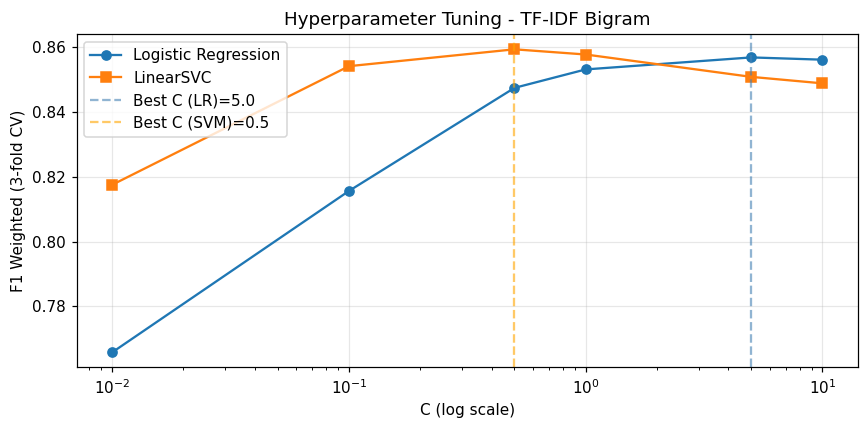
\includegraphics[width=0.85\textwidth]{07_tuning_curve.png}
\caption{Đường cong tuning tham số $C$ trên TF-IDF bigram}
\label{fig:tuning_curve}
\end{figure}

\subsection{Phân tích theo từng lớp}
Với mô hình tốt nhất (TF-IDF Bigram + SVM, $C=0.5$), chỉ số theo lớp như Bảng~\ref{tab:perclass}.

\begin{table}[H]
\centering
\caption{Precision/Recall/F1 theo lớp của mô hình tốt nhất}
\label{tab:perclass}
\begin{tabular}{lccc}
\toprule
\textbf{Lớp} & \textbf{Precision} & \textbf{Recall} & \textbf{F1} \\
\midrule
Bank account & 0.8125 & 0.8471 & 0.8294 \\
Credit card & 0.7971 & 0.8150 & 0.8059 \\
Credit reporting & 0.8378 & 0.8546 & 0.8462 \\
Debt collection & 0.8416 & 0.8120 & 0.8265 \\
Money transfer & 0.8880 & 0.8325 & 0.8594 \\
Mortgage & 0.9425 & 0.9425 & 0.9425 \\
Student loan & 0.9259 & 0.9375 & 0.9317 \\
\bottomrule
\end{tabular}
\end{table}

Lớp khó nhất là \texttt{Credit card} (F1 = 0.8059), phản ánh mức chồng lấp ngữ nghĩa với các khiếu nại \texttt{Bank account} và \texttt{Credit reporting}. Ngược lại, \texttt{Mortgage} và \texttt{Student loan} có ngôn ngữ đặc trưng rõ nên đạt F1 cao.

\begin{figure}[H]
\centering
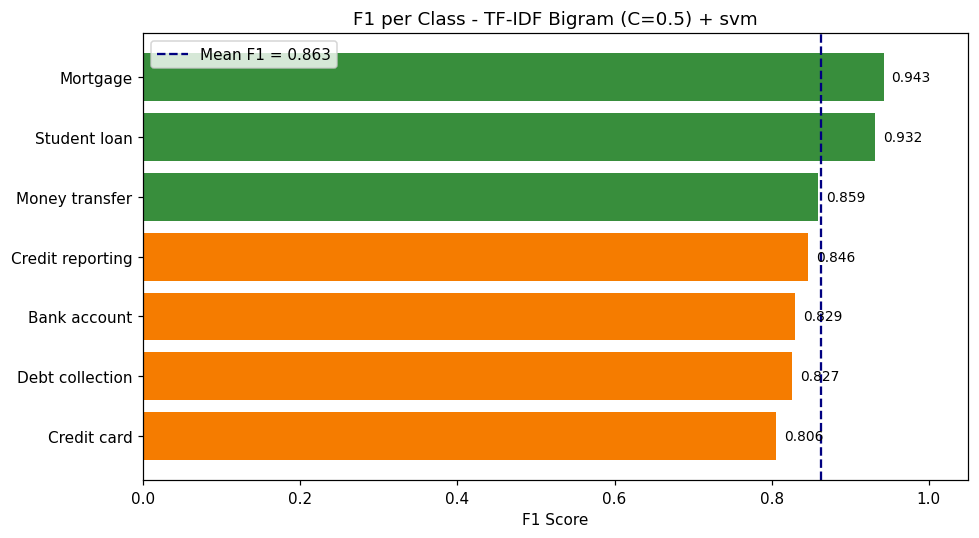
\includegraphics[width=0.95\textwidth]{10_f1_per_class.png}
\caption{Chỉ số F1-weighted chi tiết cho từng lớp của mô hình tốt nhất}
\label{fig:f1_per_class}
\end{figure}

\subsection{Phân tích ma trận nhầm lẫn và đánh đổi tốc độ-hiệu năng}
Hình~\ref{fig:cm} cho thấy phần lớn sai số tập trung ở các nhóm dịch vụ tài chính tiêu dùng gần nghĩa. Hình~\ref{fig:tradeoff} cho thấy một số mô hình BoW có thời gian huấn luyện cao nhưng không mang lại F1 tương ứng.

\begin{figure}[H]
\centering
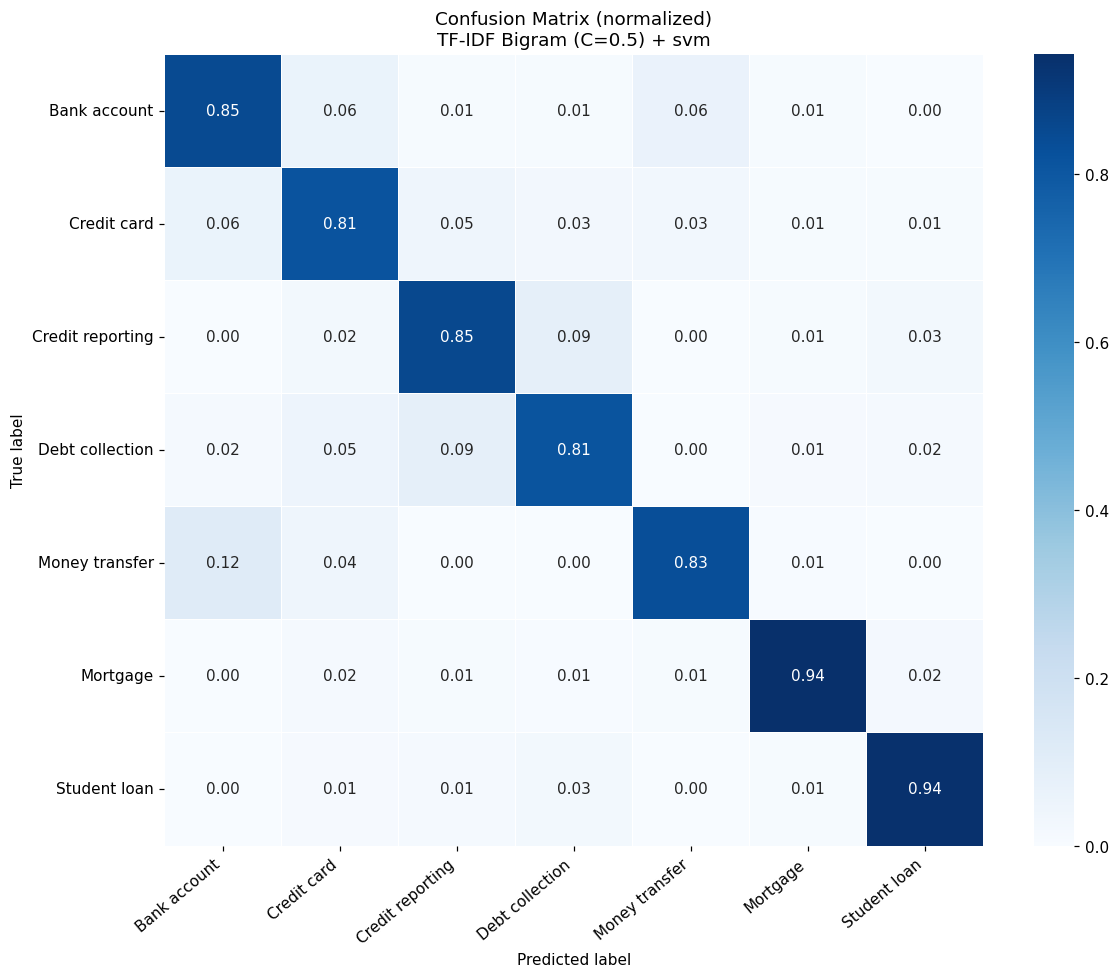
\includegraphics[width=0.9\textwidth]{09_confusion_matrix.png}
\caption{Ma trận nhầm lẫn chuẩn hóa của mô hình tốt nhất}
\label{fig:cm}
\end{figure}

\begin{figure}[H]
\centering
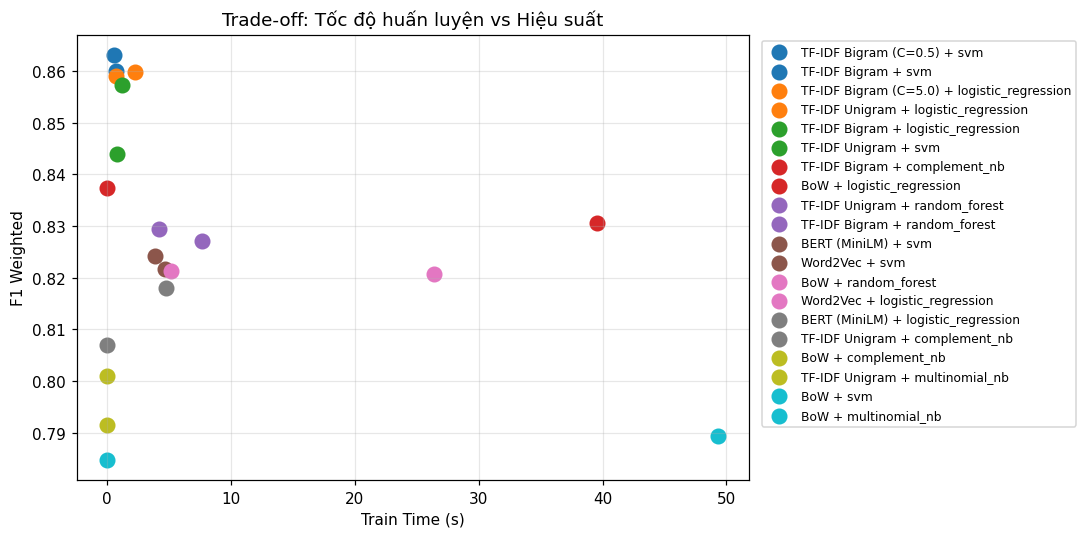
\includegraphics[width=0.95\textwidth]{11_tradeoff_time_vs_f1.png}
\caption{Trade-off giữa thời gian huấn luyện và F1-weighted}
\label{fig:tradeoff}
\end{figure}

\newpage
\section{Kết luận và hướng phát triển}

\subsection{Mức độ hoàn thành yêu cầu bài tập lớn}
Dự án đã hoàn thành các yêu cầu cốt lõi của đề bài dữ liệu văn bản:
\begin{itemize}[nosep]
    \item Thực hiện EDA và trực quan hóa phân phối dữ liệu.
    \item Xây dựng pipeline tiền xử lý văn bản có khả năng tái sử dụng.
    \item Triển khai tối thiểu hai hướng trích xuất đặc trưng (truyền thống và hiện đại).
    \item Lưu đặc trưng ra file \texttt{.npz/.npy} để tái dùng cho huấn luyện.
    \item Huấn luyện và so sánh nhiều mô hình phân loại với bộ chỉ số đầy đủ.
\end{itemize}

\subsection{Kết quả chính}
Các kết luận định lượng quan trọng:
\begin{enumerate}[nosep]
    \item Mô hình tốt nhất: \textbf{TF-IDF Bigram + LinearSVC (C=0.5)} với F1-weighted = 0.8631.
    \item Tuning tham số giúp cải thiện hiệu năng nhỏ nhưng ổn định (SVM +0.0032; LR +0.0024).
    \item Thực nghiệm cho thấy các embedding hiện đại (BERT/Word2Vec dạng feature extractor) chưa vượt qua TF-IDF bigram trong bài toán này.
    \item Sai số tập trung ở các lớp có ngữ nghĩa gần nhau, tiêu biểu \texttt{Credit card}.
\end{enumerate}

\subsection{Đóng góp kỹ thuật của hệ thống}
Bên cạnh kết quả mô hình, hệ thống có các đóng góp thực tiễn:
\begin{itemize}[nosep]
    \item Thiết kế module rõ ràng, tách được preprocessing/feature/training.
    \item Lưu đầy đủ artifact phục vụ tái lập thí nghiệm.
    \item Có sẵn unit tests cho các module trọng yếu.
    \item Notebook đáp ứng kịch bản chạy end-to-end trên nhiều nền tảng điện toán khác nhau.
\end{itemize}

\subsection{Hạn chế hiện tại}
\begin{itemize}[nosep]
    \item BERT mới dùng ở chế độ embedding tĩnh, chưa fine-tune theo miền CFPB.
    \item Chưa thực hiện calibration hoặc threshold optimization theo lớp.
\end{itemize}

\subsection{Hướng phát triển tiếp theo}
Các hướng mở rộng khả thi:
\begin{enumerate}[nosep]
    \item Fine-tune transformer trực tiếp trên bài toán phân loại 7 lớp.
    \item Thử nghiệm hybrid feature (TF-IDF + contextual embedding) và stacking.
    \item Mở rộng đánh giá với k-fold stratified và kiểm định thống kê chênh lệch mô hình.
    \item Thiết lập quy trình CI để tự động kiểm thử, tái sinh artifact và kiểm tra tính nhất quán dữ liệu.
\end{enumerate}

\newpage

\bibliographystyle{ieeetr}
\bibliography{references}

\end{document}
